\label{sec:bg}
%Rails applications are structured based on the model-view-controller
%(MVC) architecture. We illustrate this architecture in Figure~\ref{fig:ormf}. When a client requests for a URL such as {\tt http://foo.com/projects/index/1} \alvin{to make it more real how about change ... to something like foo.com}, Rails maps these requests to the controller action as shown in the Routing rules as shown in the figure \alvin{what does these rules do? is it important to know about them in this paper?}.  The mapped \alvin{?} Controller takes in the parameters from the requests and asks model to retrieve data from database. The returned data then is used to generate view which will be sent to the client side. An action is a member method of a Ruby controller class. There could exist multiple actions in a controller file to handle  different user requests. \alvin{the description here needs to map to the figure. I suggest taking a look at the description in our CIKM paper or the ICSE paper}\cong{I'll revise it.}

Rails applications are structured based on the model-view-controller (MVC) architecture. We illustrate this in Figure~\ref{fig:ormf}. When a client requests for a URL such as {\tt http://foo.com/projects/index/1} {\large \textcircled{\small 1}}, a {\it controller action} ``{\tt projects/index}'' is triggered. This action takes in the parameters from the request (e.g., ``{\tt 1}'' in the URL as {\tt params[:id]}) and interacts with the DBMS by calling the ActiveRecord API implemented by the Rails framework {\large \textcircled{\small 2}}. Rails translates the function calls into SQL queries {\large \textcircled{\small 3}}, whose results {\large \textcircled{\small 4}} are serialized into {\it model} objects (e.g., the {\tt Project} model) and returned to the controller {\large \textcircled{\small 5}}. Then, the returned objects are passed to the {\it view} {\large \textcircled{\small 6}} in order to generate a webpage {\large \textcircled{\small 7}} to send back to users {\large \textcircled{\small 8}}. Each model is derived from {\tt ActiveRecord}, and is mapped to a database table by Rails. %The data retrieval is done by translating a {\tt ActiveRecord} API call into a database query. The returned database tuples are converted into objects and sent to a {\it view} be rendered. 
A view file (ends with {\tt .erb} or {\tt .haml}) usually involves multiple languages including html, JavaScript, and ruby. The ruby code can dynamically generate the content of html elements or decide which element to show. 
%\shan{Junwen, please revise this paragraph.
%The example used here better to match an example that we will use later}

% \cong{junwen: can you change the figure, 1) reflect the data flow or the connection between MVC; 2) add the SQL query (since you estimate the SQL query time and how it contributes to a tag, I think it is important to add a concrete query in the example). 3) add circled number to the figure such that the text can easily refer, check CIKM figure2.}


% Rails maps each model class derived from {\tt ActiveRecord} to a single database table, for example a \textbf{User} class maps to the \textbf{users} table. The 
% {\tt ActiveRecord} interface also provides APIs that will be translated into
% database queries by ORM at run time.
% how the application responds to a specific web-page request. Inside
% an action there is code to retrieve database data through queries
% transparently translated by the ORM. Finally, the retrieved data is
% rendered via views that are often written in a template language, as
% shown in index.html.erb in Figure 1. Such views determine how
% the retrieved data is displayed in a client’s browser.
% The life cycle of a Rails application, and ORM applications in
% general, is as follows. When receiving a client HTTP request like
% “http://.../messages/index”, the application server first looks
% up the routing rules, shown at the top of Figure 1, to map this
% request to the index action inside MessagesController. When the
% index action executes, it invokes the @user.undeleted_messages
% function, which calls messages. where(...). The call to the Rails
% API where is dynamically translated to a SQL query by the Rails
% framework to retrieve data from the DBMS. The query results are
% then serialized into model objects and stored in @messages. The
% index action then calls render "index" to render the retrieved
% data in @messages using the index.html.erb template.

\begin{figure}[h]
    \centering
    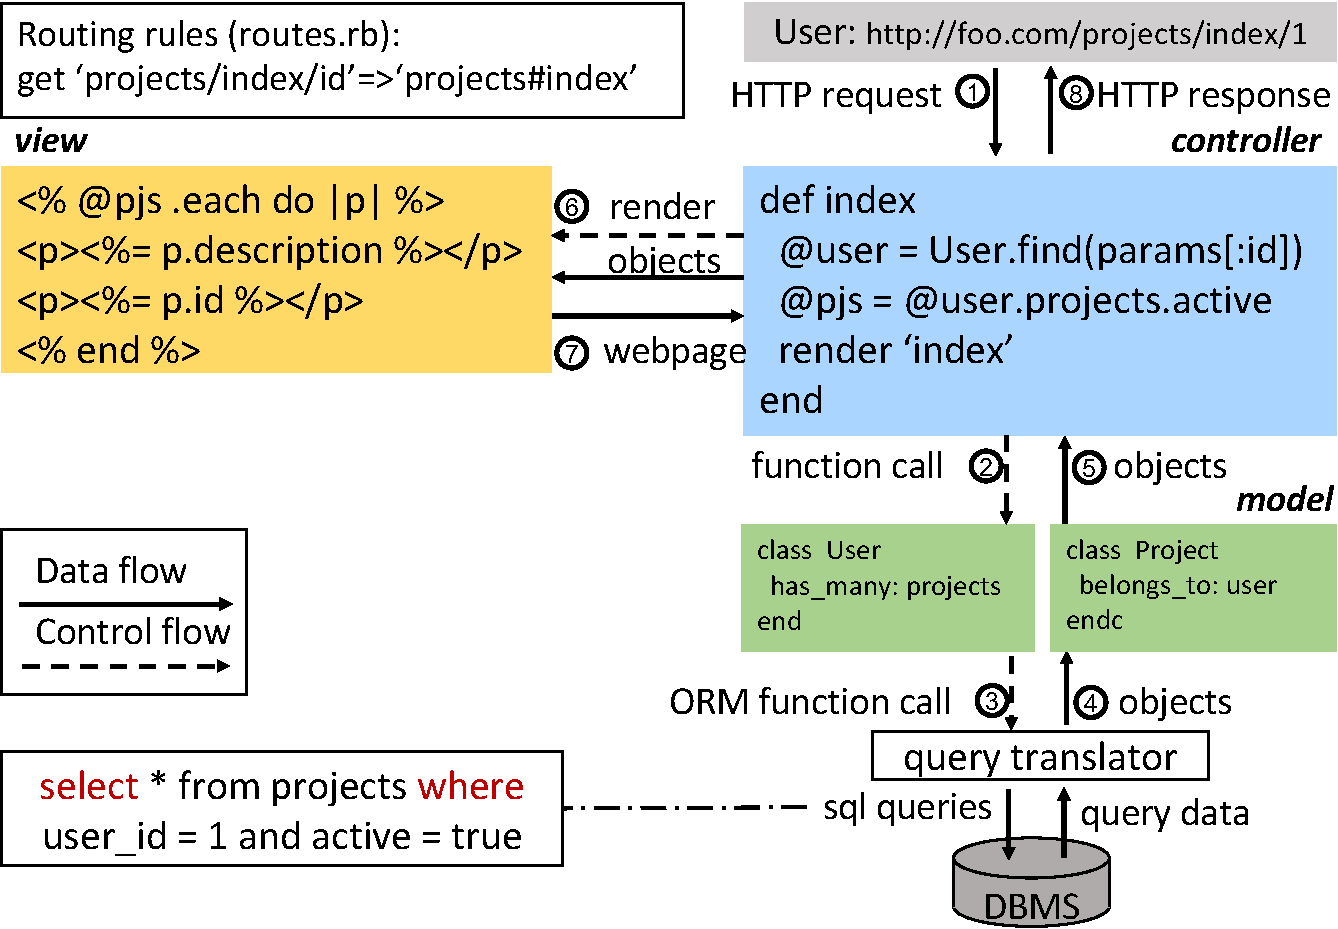
\includegraphics[width=1\columnwidth]{figs/ormf.pdf}
    \vspace{0.05in}
    \caption{Rails application architecture based on the MVC pattern}
    \label{fig:ormf}
    \vspace{-0.2in}
\end{figure}

\iffalse
% \subsection{DB-aware static analysis of Ruby on Rails}
% \label{sec:back_adg}
% During preprocessing, previous work\cong{previous, or \Tool? if previous, which work?} inlines function calls to enable inter-procedural analysis later on. This
% process involves type inference \cite{furr2009static}% xxx \shan{how?}
% , as Ruby is dynamically typed \cite{an2009static}, and special
% handling to view files and filter functions. Specifically, 
% since view files may contain computation and queries too, 
% %\Tool identifies view files rendered by each controller and appends
% %Ruby code there to the controller action. 
% \Tool extracts the ruby code in each view and inlines them to the corresponding controller where the view is rendered.
% \Tool also inlines filter functions automatically invoked before an action
% and validation functions automatically invoked before every database-modifying function. 


% Previous work~\cite{powerstation} builds the PDG for an action through the intermediate representation(IR) compiled by JRuby~\cite{jruby}. Every node $n$ in the PDG represents a statement in the JRuby IR and 
% every edge $e$ represents either control dependency or data dependency. Furthermore, a data-dependency
% edge $n_1 \rightarrow n_2$ indicates that the output object $o$ of $n_1$ is used by $n_2$ without
% other statements overwriting $o$ in between. For each statement, we keep the line number information. Combining with the APIs provided by ActiveRecord and the database schema information, we further decide whether a node is a query. 

% The PDG generated above is then extended in three ways to create the ADG: 
% (1) changing and splitting some nodes to become 
% Query nodes; (2) annotating every Query node with the database table and fields that are read or written; 
% (3) annotating every outgoing data-dependency edge of a Query node with the exact field(s) that are used.

% To accomplish this, previous work first analyzes every model class that extends the Rails
% {\tt ActiveRecord} interface to determine all the database
% tables in the application and the association relationship among them.
% For example, analyzing the model classes illustrated in 
% Figure~\ref{fig:schema}, \Tool identifies the {\tt users} table
% corresponding to the {\tt User} class and similarly for the {\tt Blog} class, and that these two models have 
% a one-to-many relationship, i.e., each instance of {\tt User} may own multiple instances of {\tt Blog}.
% Second, \Tool analyzes the {\tt schema.rb} file to determine
% how many fields each table contains. For example, parsing the
% {\tt schema.rb} snippet in Figure~\ref{fig:schema}, \Tool learns about 
% the schemas of table {\tt users} and {\tt blogs} as
% shown in the bottom of the figure.

% Third, \Tool identifies queries from three sources: (1) explicit 
% invocations of
% Rails {\tt ActiveRecord} Query APIs, such as {\tt exist?},
% {\tt reload}, \textit{\tt update}, \textit{\tt destroy}, etc;
% (2) implicit queries generated by Rails to access object fields, e.g., {\tt $o_1$.$o_2$}, where 
% the class of $o_1$ and the class of $o_2$ are associated model classes
% (e.g., {\tt user.blogs} would incur a query to
% retrieve records in {\tt blogs} table that are associated with
% the specific {\tt user} record in {\tt users} table);
% (3) explicitly invoked raw SQL queries through  Base.connection.execute.
% %\junwen{it's also thru the ActiveRecord API, similar as the first type}
% Any query identified above is represented as a Query node in the ADG.\footnote{At run time,
% multiple such queries could be composed by ORM into one SQL query.
% Such query chaining does not affect \Tool analysis.} 

\fi